% PLANTILLA APA7
% Creado por: Andres Bergsneider
% GNU General Public License
% Última actualización: 23/07/2021

%------------------------------------------------------
%	Preámbulo
\documentclass[doc, 12pt, letterpaper, donotrepeattitle, floatsintext, apacite]{apa6}    % Was apa7, apa6 works better for citations [AB]
\usepackage[utf8]{inputenc}
\usepackage{comment}
\usepackage{marvosym}
\usepackage{graphicx}
\usepackage{float}
\usepackage[normalem]{ulem}
\usepackage[spanish]{babel}
\usepackage{setspace}
\usepackage{xspace} % Para forzar espacios [AB]
\usepackage[colorinlistoftodos]{todonotes}  % Paquete para comentarios! [AB]
\usepackage{amsmath} % Para Matrices y ecuaciones [AB]
%\usepackage{hyperref} % need to fix, causes issues [AB]

\selectlanguage{spanish}
\useunder{\uline}{\ul}{}
\newcommand{\myparagraph}[1]{\paragraph{#1}\mbox{}\\}
\newcommand{\latex}{\LaTeX\xspace}  % para simplificar el uso de \LaTeX
%------------------------------------------------------
%	Portada
%\thispagestyle{empty}
\title{\Large Manuscrito Estilo APA6/7}
\shorttitle{Reflexión sobre la actual situación en Colombia}
\author{Nombre del Autor} 
\affiliation{Nombre de Organización\\ Materia en Curso\\ Código: 123456789}
%\course{Código: 201923806}
%\professor{Nombre del docente}
%\duedate{Fecha}
%------------------------------------------------------

% De aquí para abajo empieza el documento [AB]
\begin{document}
\vspace*{-2cm}      % removes vertical space on title section [AB]
\maketitle          % PORTADA, quitar "%" al principio para activar

%------------------------------------------------------
%	Índices
%\pagenumbering{roman}
    % Contenido
%\renewcommand\contentsname{\largeÍndice}
%\tableofcontents
%\setcounter{tocdepth}{2}
%\newpage
    % Fíguras
%\renewcommand{\listfigurename}{\largeÍndice de fíguras}
%\listoffigures
%\newpage
    % Tablas
%\renewcommand{\listtablename}{\largeÍndice de tablas}
%\listoftables
%\newpage
%------------------------------------------------------
%   Cuerpo
\pagenumbering{arabic}

%\section{\large Reflexión sobre la actual situación en Colombia}
\doublespacing % espacio entre renglón doble [AB]

% Abstracto
Aquí viene el abstracto...


\section{\large Introducción}
Aquí se escribe la introducción de la investigación. A continuación habrán ejemplos de varios comandos y características especiales de \latex

\section{\large Algunos Ejemplos}

\subsection{Sección}
Usa los comandos \verb|\section| y \verb|\subsection| para organizar tu documento. \latex te organiza todo tu formato y numeraciones automáticamente. Usa los comandos \verb|\ref| y \verb|\label| para hacer referencias.

\subsection{Comentarios} 
He agregado el paquete \verb|\usepackage[colorinlistoftodos]{todonotes}| para permitir el uso de notas dentro del texto.
\todo[inline, color=green!40]{Este es un ejemplo :)}


\subsection{Referencias} 
Este documento de \latex esta configurado para usando el estándar de APA6 con modificaciones de APA7. \latex automáticamente genera la bibliografía en este estilo siempre y cuando la escribas dentro del archivo \textbf{mibibliografia.bib}. Usando el comando \verb|\cite| se genera la citación en paréntesis. \latex fue desarrollado por Leslie Lamport en 1986 \cite{lamport1986}.

\subsection{Cuadros e Imágenes}
Usa el comando \verb|\begin{table}| para crear cuadros. En el Cuadro \ref{cuadro:ejemplo} se  observa un ejemplo.
Para el uso de imagenes, usar el comando \verb|\begin{figure}|, es necesario tener el paquete \verb|\begin{figure}|. La Imagen \ref{imagen:ejemplo} da un ejemplo de su uso.

\begin{table}[h] % el [h] es para posicionar el cuadro aquí. Mas de esto en los links del README.md
    \centering
    \begin{tabular}{l|r}
        Item & Quantity \\\hline
        Widgets & 42 \\
        Gadgets & 13
    \end{tabular}
    \caption{Aqui va la leyenda del cuadro}
    \label{cuadro:ejemplo}
\end{table}

\begin{figure}[H]
    \centering
    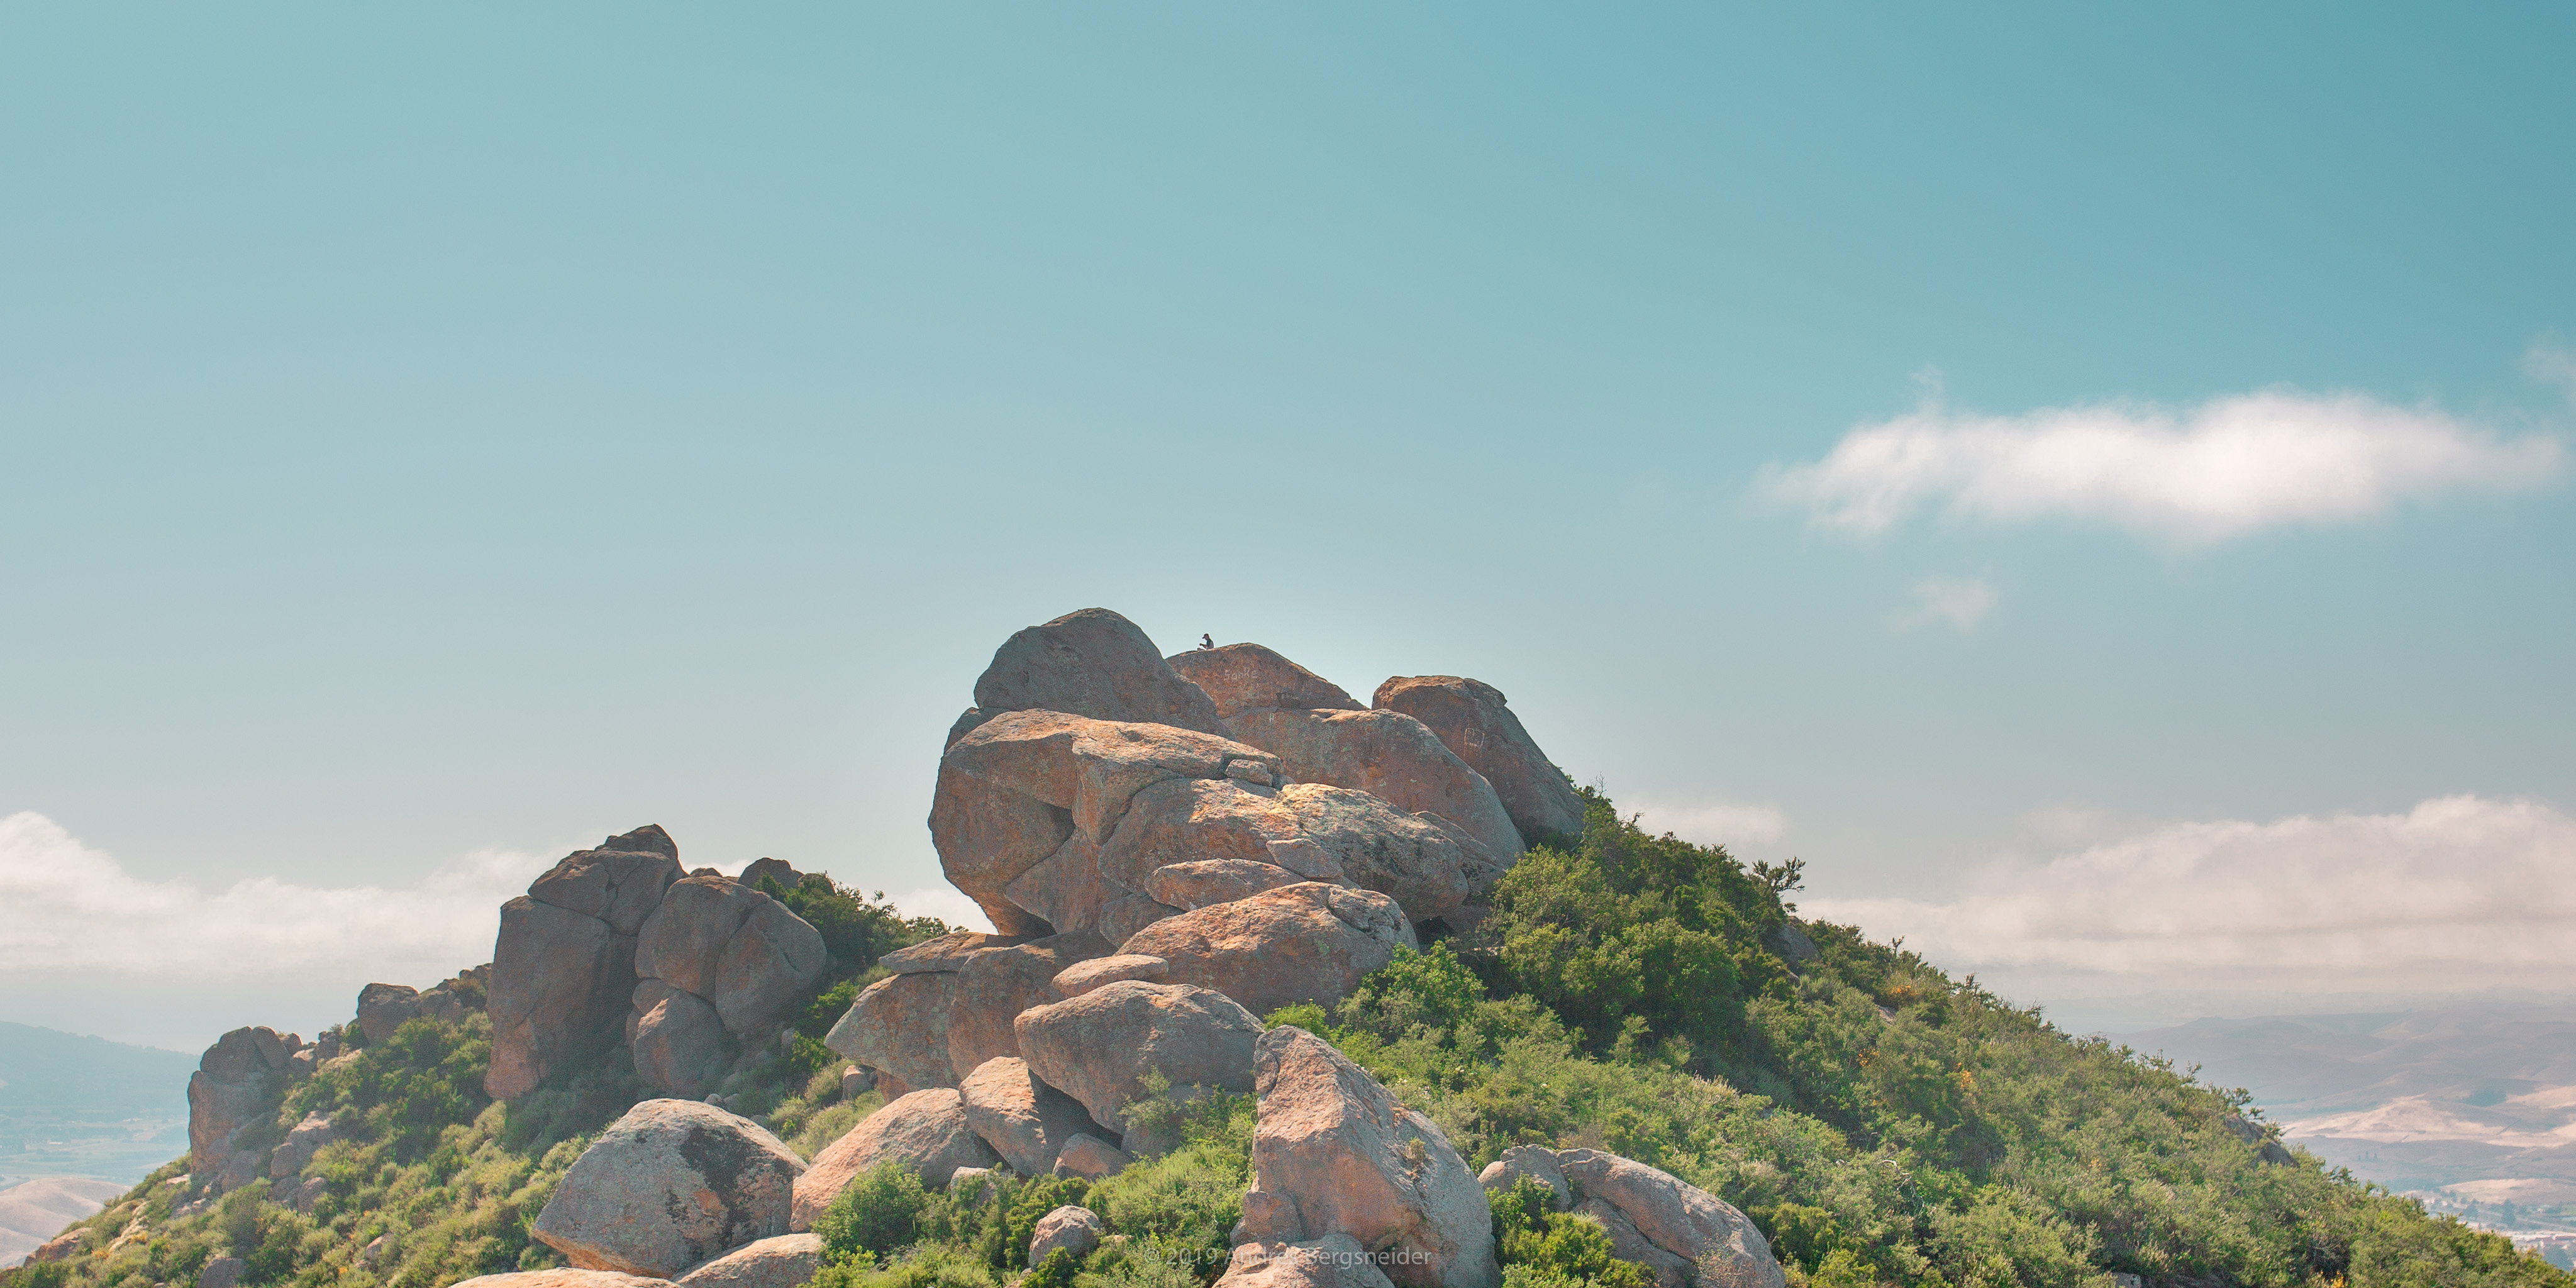
\includegraphics[width=.7\textwidth]{Imágenes/ARB-7747.jpg}
    \caption{Créditos: Andres Bergsneider}
    \label{imagen:ejemplo}
\end{figure}


\subsection{Listas}
Asimismo, hay varios tipos de listas. Lista tipo \textit{bullet-points} y listas enumeradas, usando los comandos \verb|\begin{itemize}| y \verb|\begin{enumerate}| respectivamente.

\begin{itemize}
    \item Así
    \item Y así
\end{itemize}

Listas enumeradas:

\begin{enumerate}
    \item Así
    \item Y así
\end{enumerate}

\subsection{Ecuaciones}
Por ultimo, les dejo el ejemplo de uso de ecuaciones, usando el comando \verb|\begin{equation}|.

\begin{equation}
    S = \frac{1}{90} \sum_{i=210}^{299} \left(\frac{|P^{(i)}_k \cap T^{(i)}_k|}{|P^{(i)}_k| + |T^{(i)}_k|} + \frac{|P^{(i)}_t \cap T^{(i)}_t|}{|P^{(i)}_t| + |T^{(i)}_t|}\right)
    \label{dice}
\end{equation}

Y un ejemplo usando matrices, aquí es necesario el comando \verb|\begin{bmatrix}|:

    \begin{equation}
    \label{eqn:convolution}
    \renewcommand{\arraystretch}{0.8}
    \vec{x}*\vec{a} = X\vec{a} =
        \begin{bmatrix}
           x    &   y   &   x   &   0   &   0   &   0 \\
           0    &   0   &   x   &   y   &   x   &   0 
        \end{bmatrix}
        \begin{bmatrix}
           0\\
           a\\
           b\\
           c\\
           d\\
           0
        \end{bmatrix}
    = 
        \begin{bmatrix}
           ay+bz\\
           bx+cy+dz
        \end{bmatrix}
\end{equation}


\newpage
% Referencias
\renewcommand\refname{\large\textbf{Referencias bibliográficas:}}
\bibliography{mibibliografia}

\end{document}